\documentclass[12pt]{beamer}
\usetheme{Warsaw}
\usepackage[utf8]{inputenc}
\usepackage{amsmath}
\usepackage{amsfonts}
\usepackage{amssymb}
\usepackage{graphicx}
\usepackage[font=Times,timeinterval=1,timeduration=2.0,timedeath=0,fillcolorwarningsecond=white!60!yellow,timewarningfirst=50,timewarningsecond=80,resetatpages=2]{tdclock}
\usepackage{tabularx}
\usepackage{array}
\usepackage{multicol}
\usepackage{longtable}
\usepackage{xcolor}
\usepackage{gensymb}
\usepackage{pgfplots}
\usepackage[makeroom]{cancel}

\graphicspath{ {./references/} }
\pgfplotsset{
	soldot/.style={color=black,only marks,mark=*},
	holdot/.style={color=black,fill=white,only marks,mark=*},
	compat=1.12
}
\newcolumntype{Y}{>{\centering\arraybackslash}X}
\makeatletter
\def\@listii{\leftmargin\leftmarginii
			  \topsep    2ex
			  \parsep    0\p@   \@plus\p@
			  \itemsep   \parsep}
\makeatother

\begin{document}
\begin{frame}
	\frametitle{Bellwork 9/18}
	\initclock
	Let $g$ and $h$ be the functions defined by: \[g(x) = \sin\left[\frac{\pi}{2}(x+2)\right] + 3 \text{; } h(x) = -\frac{1}{4}x^3-\frac{3}{2}x^2-\frac{9}{4}x+3\]\par
	If $f$ is a function that satisfies \[g(x)\leq f(x)\leq h(x) \text{ for } -2 < x < 0\text{,}\]\par
	what is $\displaystyle\lim_{x\to-1}f(x)$?
	\begin{enumerate}\itemsep0.5ex
		\item $3$
		\item $3.5$
		\item $4$
		\item The limit cannot be determined from the information given.
	\end{enumerate}
	\crono
	\resetcrono{\beamerbutton{reset}}
\end{frame}
\begin{frame}
	\frametitle{Bellwork 9/18 - Solution}
	\large
	\vspace*{\fill}
	\vspace*{\fill}
	\vspace*{\fill}
	\vspace*{\fill}
	\[g(x)\leq f(x)\leq h(x)\]
	\vspace*{\fill}
	\[\displaystyle\lim_{x\to-1}g(x)\leq \displaystyle\lim_{x\to-1}f(x)\leq \displaystyle\lim_{x\to-1}h(x)\]
	\vspace*{\fill}
	\[4=\displaystyle\lim_{x\to-1}f(x)=4\]
	\vspace*{\fill}
	\[\implies\boxed{\displaystyle\lim_{x\to-1}f(x)=4}\]
	\vspace*{\fill}
	\vspace*{\fill}
	\vspace*{\fill}
	\vspace*{\fill}
\end{frame}
\begin{frame}
	\frametitle{Exercise 1}
	\large
	\[f(x) = \frac{|x|}{x}+\frac{x^2-4}{x-2}+\frac{1}{x-4}\]\par
	\vspace*{\fill}
	What type of discontinuity exists at,\par
	\vspace*{\fill}
	\begin{enumerate}\itemsep2ex
		\item{
		            \begin{center}
			            $x = 0$
		            \end{center}
		      }
		\item{
		            \begin{center}
			            $x = 2$
		            \end{center}
		      }
		\item{
		            \begin{center}
			            $x = 4$
		            \end{center}
		      }
	\end{enumerate}
\end{frame}
\begin{frame}
	\frametitle{Exercise 1 - Solutions}
	% https://www.desmos.com/calculator/fpvvpgmm03

	\begin{center}
		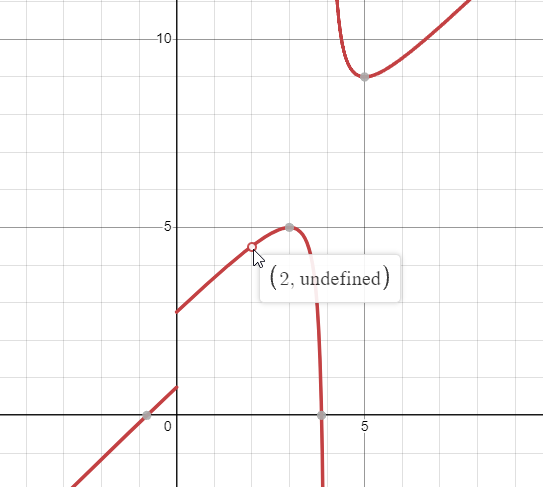
\includegraphics[scale=0.6]{exercise_1_solution_graph.png}
	\end{center}
\end{frame}
\begin{frame}
	\frametitle{Exercise 2}
	\Large
	\begin{center}
		Let $f(x) =
			\begin{cases}
				ax + 1 & \text{if } x < 2    \\
				ax^2   & \text{if } x \geq 2 \\
			\end{cases}
		$\\
		\vspace*{\fill}
		For what value $a$ is $f(x)$ continuous?
	\end{center}
\end{frame}
\begin{frame}
	\frametitle{Exercise 2 - Solutions}
	% https://www.desmos.com/calculator/gq2nkmhgxn

	\large
	\begin{center}
		$f(x) =
			\begin{cases}
				ax + 1 & \text{if } x < 2    \\
				ax^2   & \text{if } x \geq 2 \\
			\end{cases}
		$\\
		\vspace*{\fill}
	\end{center}
	For $f(x)$ to be continuous,
	\[\displaystyle\lim_{x\to2^{-}}f(x)=\displaystyle\lim_{x\to2^{+}}f(x)=f(2)\]
	\[\implies a(2)+1 = a(2^2)\]
	\[\implies 1 = 2a\]
	\[\implies \boxed{a = \frac{1}{2}}\]
\end{frame}
\begin{frame}
	\frametitle{Exercise 3}
	\large
	\begin{center}
		Let $g(x) =
			\begin{cases}
				be^{\frac{2x}{\pi}}-2 & \text{if } x < \frac{\pi}{2}    \\
				b\sin(x)              & \text{if } x \geq \frac{\pi}{2} \\
			\end{cases}
		$\\
		\vspace*{\fill}
		\Large
		For what value $b$ is $g(x)$ continuous?
	\end{center}
\end{frame}
\begin{frame}
	\frametitle{Exercise 3 - Solutions}
	% https://www.desmos.com/calculator/tqvetoqbxv

	\large
	\begin{center}
		$g(x) =
			\begin{cases}
				be^{\frac{2x}{\pi}}-2 & \text{if } x < \frac{\pi}{2}    \\
				b\sin(x)              & \text{if } x \geq \frac{\pi}{2} \\
			\end{cases}
		$\\
		\vspace*{\fill}
	\end{center}
	For $g(x)$ to be continuous,
	\[\displaystyle\lim_{x\to\frac{\pi}{2}^{-}}g(x)=\displaystyle\lim_{x\to\frac{\pi}{2}^{+}}g(x)=g\left(\frac{\pi}{2}\right)\]
	\[\implies be^{\frac{2}{\pi}\cdot\frac{\pi}{2}}-2 = b\sin\left(\frac{\pi}{2}\right)\]
	\[\implies be^1 - 2 = b\]
	\[\implies b(e-1) = 2\]
	\[\implies \boxed{b = \frac{2}{e-1}}\]
\end{frame}
\end{document}